\documentclass{svjour3}                     % onecolumn (standard format)
\smartqed  % flush right qed marks, e.g. at end of proof
\usepackage{graphicx}
\usepackage{enumerate}
\usepackage{amssymb,amsmath}
\usepackage{mathptmx}     
\journalname{MISTA 2015}

% Our commands
\usepackage{todonotes}
%\newcommand{\cNP}{$\mathcal{NP}$}
%\newcommand{\cP}{$\mathcal{P}$}

\begin{document}
	
\title{Scheduling a conference to minimize RSVP conflicts}
\author{Jeffrey Quesnelle \and Daniel Steffy}
	
\institute{Jeffrey Quesnelle \at
	Oakland University \\
	\email{jfquesne@oakland.edu}           %  \\
	\and
	Daniel Steffy \at
	Oakland University \\
	\email{steffy@oakland.edu}           %  \\
}

\maketitle
	
\begin{abstract}
This paper describes a conference scheduling (or timetabling) problem where, at the time of registration, participants RSVP to events which they would like to attend.
Based upon these preferences, an assignment of events to rooms and time slots should be determined that minimizes the number of RSVP conflicts and satisfies a number of hard constraints.
We show that our problem, and several variants of it, are NP-hard.
An integer programming model is developed to solve the problem and a computational study of this model is performed on instances generated from real data.
Improvements to the model, including a symmetry breaking reformulation and a dualization of some hard constraints, are shown to significantly improve solution times, making the problem tractable for the desired real world application.
\end{abstract}

\section{Introduction}


This project was motivated by the problem of scheduling events within PenguiCon \cite{pc}, a conference organized by the open-source community in Michigan.  
The conference typically includes approximately 250 events such as lectures, demonstrations and panel discussions, all of which must be scheduled into rooms and time slots.
Many of the events involve multiple presenters/panelists, and many presenters participate in more than one event; it is a hard constraint that no speaker can be multi-booked during a given time period.
Furthermore, the registration website will give conference participants the ability to ``RSVP" to events before the schedule is generated, giving the extra complication of trying to generate the schedule based on these RSVPs that minimizes conflicts amongst presentations that attendees had previously indicated a common interest.
Our problem is related to previously studied conference and class scheduling problems but includes what we believe is a novel and difficult combination of constraints and objectives.
The goal of this paper is to model our problem, relate it to previous work, and implement solution methods that can be deployed to schedule the PenguiCon conference in practice.

In Section~\ref{sec.back} we discuss some related work.
In Section~\ref{sec.desc} we formally describe our problem and relate it to previous work,
we also show that our scheduling problem, and some variants, are all NP-hard.
Section~\ref{sec.model} describes an integer programming model for the problem.
Various improvements to the model are also described and evaluated computationally.
Section~\ref{sec.conclusion} provides concluding remarks.

\section{Background and related work}\label{sec.back}

One of the oldest scheduling problems that has been studied is the \emph{timetable design problem} (TTD). 
Given a set of time slots, a set of teachers and their available teaching hours, and a matrix describing which courses each teacher is required to teach,  the TTD problem is the problem of determining if there exists a schedule that satisfies the constraints. 
TTD was shown to be NP-Complete in 1976 via reduction from 3-SAT \cite{even76}. 
However it is notable that certain variants of the TTD problem are known to be polynomial time solvable. 
For example, if each teacher is only available for up to two hours, or each teacher is able to teach any class, then the problem is solvable in polynomial time \cite{garey76}.

The basic TTD model often doesn't map well onto several common problems such as scheduling courses for a university. 
Specifically, the requirement that a teacher \emph{must} teach certain classes may be relaxed to describing those classes they are \emph{willing} to teach. 
This is know as the Basic Course Scheduling problem (BCS); it was shown to be solvable in polynomial time by Lovelace~\cite{lovelace2010}. 
Extensions of the BCS, for example including the requirement that courses are assigned to rooms, results again in an NP-hard problem.

The scheduling problem considered in this paper more closely resembles the TTD problem, before introducing it we will give a precise formulation of the TTD.
Here we denote the decision variables as a function $f$, which gives the assignment of presenters to talks and hours.
We henceforth refer to the courses, or events as \emph{talks}.
We also assume that all talks have the same length and introduce a set of \emph{hours} which is used to represent the set of time slots in which talks can be scheduled.

\begin{quote}
	\textsc{Timetable Decision Problem}
	
	\underline{INSTANCE}:
	\begin{enumerate}
		\item a finite set $H$ of hours and numbers $n$ and $m$ indicating the number of presenters and talks, respectively; 
		\item a collection $P = \{P_1, P_2, \cdots, P_n\}$, where $P_i \subseteq H$ (there are $n$ presenters and $P_i$ is the set of hours during which the $i$th presenter is available for presenting);
		\item a collection $T = \{T_1, T_2, \cdots, T_m\}$, where $T_j \subseteq H$ (there are $m$ talks and $T_j$ is the set of hours during which the $j$th talk can be given);
		\item an $n \times m$ matrix $G$ of nonnegative integers ($G_{ij}$ is the number of hours (times) which the $i$th presenter will give the $j$th talk).
	\end{enumerate}
	\underline{QUESTION}: Does there exist a function 
	\begin{gather*}
		f(i,j,h) : \{1,\cdots,n\} \times \{1,\cdots,m\} \times H \rightarrow \{0,1\}
	\end{gather*}
	(where $f(i,j,h)=1$ if and only if presenter $i$ gives talk $j$ during hour $h$) such that
	\begin{enumerate}[(a)]
		\item $f(i,j,h) = 1 \Rightarrow h \in P_i \cap T_j$ (the presenter and talk are both available to be scheduled at hour $h$);
		\item $\sum\limits_{h \in H} f(i,j,h) = G_{ij}$ for all $1 \le i \le n$ and $1 \le j \le m$ (the $i$th presenter was scheduled for the $j$th talk the required number of times);
		\item $\sum\limits_{i=1}^n f(i,j,h) \le 1$ for all $1 \le j \le m$ and $h \in H$ (no talk has more than one presenter at a time);
		\item $\sum\limits_{j=1}^m f(i,j,h) \le 1$ for all $1 \le i \le n$ and $h \in H$ (no presenter is giving more than one talk simultaneously).
	\end{enumerate}
\end{quote}


\section{Conference scheduling problem}\label{sec.desc}
We now consider extensions and modifications of the TTD problem that incorporate requirements arising from our application.

\subsection{Conference TTD Problem}
Although the TTD problem is related to our target problem, it does not capture all of the decisions and constraints involved.
One requirement is that some talks may involve multiple presenters, each of which may have additional differing scheduling conflicts.
In the TTD model constraint (c) ensures that each talk is scheduled to exactly one presenter. 
In the case where multiple presenters are allowed we most likely wish to add a different constraint: that for each talk \emph{every} presenter that can be scheduled is scheduled. 
For example, if Alice is giving talks A, B, and C, and Bob is giving talks B, C, and D, all scheduled instances of B and C should include both Alice and Bob. 
We call this variant the Conference Timetable Decision problem (CTTD).
\begin{quote}
	\textsc{Conference Timetable Decision Problem}
	
	Same as TTD, but with constraint (c) changed to
	\begin{enumerate}[(c)]
		\item ($G_{ij} > 0) \land (G_{i'j} > 0) \Rightarrow f(i,j,h)=f(i',j,h)$ for all $1 \le i,i' \le n$, $1 \le j \le m$ and $h \in H$ (all presenters that are required to give a talk must be present at all instances of that talk);
	\end{enumerate}
\end{quote}

We now show that CTTD is NP-complete via reduction from the Graph $k$-colorability problem, the decision problem of determining whether a graph admits a $k$-coloring, which is well known to be NP-complete \cite{garey76_2}.
As we will see in the proof, the CTTD problem is NP-complete even without the inclusion of the availability constraints and even if each entry $G_{ij}$ is equal to zero or one.
%We note that although result is not surprising, it does not follow trivially via reduction from TTD.

\begin{proposition}\label{cttd_np}
	CTTD is NP-Complete.
\end{proposition}
\begin{proof}
We first note that CTTD is clearly in NP.  
Given a graph $G=(V,E)$ and a positive integer $k$, we will show how to construct an instance of CTTD that is feasible if and only if $G$ is $k$-colorable.
For simplicity of presentation we assume that $G$ contains isolated nodes (coloring of such nodes is trivial).
Essentially, a talk is created to correspond to each vertex in $G$, each of the $k$ colors corresponds to an hour in which talks can be scheduled and speakers are created to correspond to the edges in $G$.
More formally, define $H=\{1, 2, \cdots, k\}$ and for each vertex $v_j \in V=\{v_1, v_2, \cdots, v_{|V|}\}$ let $T_j = H$. 
For each edge $e_l \in E=\{e_1, e_2, \cdots, e_{|E|}\}$ we let $P_l = H$. 
For each $e_l = (v_i,v_j)\in E$, where $v_i,v_j \in V$, we let $\hat G_{li} = \hat G_{lj} = 1$, and let $\hat G_{lm}=0$ for each $m\neq i,j$. 
%Finally, for each node $v_i\in V$ with degree zero in $G$, we create an additional speaker $l$ with $\hat G_{li} = 1$ and $\hat G_{lk}=0$ for other values of $k$, this is simply to ensure that each talk has a speaker and will be assigned a time slot in a feasible schedule.
We now have an instance $(H, P, T, \hat G)$ of CTTD (whose construction was easily computed in polynomial time). 

We now observe that $(H, P, T, \hat G)$ has a feasible schedule $f$ if and only if $G$ is $k$-colorable.
Given a feasible schedule $f$, each vertex $v_a$ in $G$ is assigned color $h$, where $h$ is the timeslot in which talk $a$ is assigned.
For any edge $e_l=(v_i,v_j)\in E$ we note that since a speaker $l$ was created to give talks $i$ and $j$ they will not be scheduled in the same time slots, and thus $v_i,v_j$ are assigned different colors, leading to a valid $k$-coloring of $G$.
Conversely, given a $k$-coloring of $G$ it is easy to construct a feasible schedule $f$ for $(H, P, T, \hat G)$ using the same idea.
Finally we conclude that CTTD is NP-Complete.
\end{proof}


\subsection{Basic Conference TTD Problem}
Lovelace showed that a relaxed version of TTD (called BCS for ``Basic Course Scheduling") can be solved in polynomial time using a network flow model \cite{lovelace2010}. 
The principal differences between BCS and TTD are the reduction of many ``hard" requirements such as those insisting that presenters give \emph{exactly} a certain number of talks of a certain type to simply saying they may give \emph{at most} the number of talks for which they are \emph{willing} to give. 
BCS does maintain a hard requirement that all presentations must be scheduled, but offers flexibility in which speaker makes each presentation.
We give a formulation of BCS using notation consistent with our description of the Basic Timetable Decision Problem (BTTD).

\begin{quote}
	\textsc{Basic Timetable Decision Problem}
	
	\underline{INSTANCE}:
	\begin{enumerate}
		\item a finite set $H$ of hours and numbers $n$ and $m$ indicating the number of presenters and talks, respectively; 
		\item a collection $P = \{P_1, P_2, \cdots, P_n\}$, where $P_i \subseteq H$ (there are $n$ presenters and $P_i$ is the set of hours during which the $i$th presenter is available for presenting);
		\item a collection $T = \{T_1, T_2, \cdots, T_m\}$, where $T_j \subseteq H$ (there are $m$ talks and $T_j$ is the set of hours during which the $j$th talk can be given);
		\item a function $L : \mathbb Z^+ \rightarrow \mathbb Z_0^+$, where $L(n)$ is the maximum number of talks that the $n$th presenter can give;
		\item a function $S : \mathbb Z^+ \rightarrow \mathbb Z_0^+$, where $S(m)$ is the desired number of instances of the $m$th presentation;
		\item a function $WTP : \{1,2,\cdots, n\} \times \{1,2,\cdots,m\} \rightarrow \{0,1\}$, where $WTP(i,j)$ indicates if the $i$th presenter is Willing To Present the $j$th talk.
	\end{enumerate}
	\underline{QUESTION}: Does there exist a function 
	\begin{gather*}
		f(i,j,h) : \{1,\cdots,n\} \times \{1,\cdots,m\} \times H \rightarrow \{0,1\}
	\end{gather*}
	(where $f(i,j,h)=1$ if and only if presenter $i$ gives talk $j$ during hour $h$) such that
	\begin{enumerate}[(a)]
		\item $f(i,j,h) = 1 \Rightarrow h \in P_i \cap T_j$ (the presenter and talk are both available to be scheduled at hour $h$);
		\item $\sum\limits_{h \in H} f'(j,h) = S(j)$ for all $1 \le j \le m$ where $f'(j,h) = 1 \iff \exists i \text{ with } 1 \le i \le n$ such that $f(i,j,h)=1$, and 0 otherwise (the $j$th talk is given the required number of times);
		\item $\sum\limits_{j=1}^{m} f(i,j,h) \le 1$ for all $1 \le i \le n$ and $h \in H$ (there is no more than one presenter scheduled for each instance of a talk);
		\item $f(i,j,h) = 1 \Rightarrow WTP(i,j) = 1$ (only presenters willing to give a talk are scheduled for it);
		\item $\sum\limits_{j=1}^n\sum\limits_{h \in H} f(i,j,h) \le L(i)$ for all $1 \le i \le n$ (the total number of talks that the $i$th presenter is scheduled for is at most their maximum number of presentations)
		\item $\sum\limits_{j=1}^m f(i,j,h) \le 1$ for all $1 \le i \le n$ and $h \in H$ (no presenter is giving more than one talk simultaneously).
	\end{enumerate}
\end{quote}
\begin{remark}
	BTTD $\in$ P \cite{lovelace2010}.
\end{remark}
The difference between TTD and CTTD is the ability for presentations to have multiple presenters, and the requirement that all presenters be scheduled for all instances of a talk. 
Likewise, we can formulate a modified version of BTTD that incorporates this new constraint which we will call the Basic Conference Timetable Decision problem (BCTTD). 
\begin{quote}
	\textsc{Basic Conference Timetable Decision Problem}
	
	Same as BTTD, but with constraint (c) changed to
	\begin{enumerate}[(c)]
		\item $WTP(i,j) = WTP(i',j) \Rightarrow f(i,j,h)=f(i',j,h)$ for all $1 \le i,i' \le n$, $1 \le j \le m$ and $h \in H$ (all presenters that are required to give a talk must be present at all instances of that talk);
	\end{enumerate}
\end{quote}

We observe that after this constraint is introduced, we may apply the same reduction used in Proposition~\ref{cttd_np} and thus we have the following.

\begin{proposition}\label{bcttd_np}
	BCTTD is NP-Complete.
\end{proposition}

%Perhaps somewhat surprisingly the mere modification of requirement (c) in BTTD to our stronger version in BCTTD is enough to move the problem from P into NP-Complete. \\

\subsection{Extended Conference TTD Problem}
We now present a modification to CTTD that introduces room assignment decisions and room compatibility constraints.
The CTTD problem assigns speakers to talks and time slots but, as in many other applications, we also require that talks are assigned to suitable rooms.
Furthermore, rooms also may only be available during certain times or suitable for certain talks and this information must be factored into the problem. 
This leads us to the Extended Conference Timetable Decision problem (ECTTD).
\begin{quote}
	\textsc{Extended Conference Timetable Decision Problem}
	
	\underline{INSTANCE}: Same as CTTD, but with the additional parameters:
	\begin{enumerate}[1.]
		\setcounter{enumi}{4}
		\item a finite set $R$ of rooms;
		\item a collection $\{A_1,A_2,\cdots,A_r\}$, where $A_k \subseteq H$ (there are $r=|R|$ rooms and $A_k$ is the set of hours during which the $k$th room is available);
		\item a collection $\{S_1,S_2,\cdots,S_m\}$, where $S_l \subseteq R$ (there are $m$ talks and $S_l$ is the set of rooms that the $l$th presentation may be given in)
	\end{enumerate}
	\underline{QUESTION}: Does there exist a function 
	\begin{gather*}
		f(i,j,h,r) : \{1,\cdots,n\} \times \{1,\cdots,m\} \times H \times R \rightarrow \{0,1\}
	\end{gather*}
	(where $f(i,j,h,r)=1$ if and only if presenter $i$ gives talk $j$ during hour $h$ in room $r$) such that
	\begin{enumerate}[(a)]
		\item $f(i,j,h,r) = 1 \Rightarrow h \in P_i \cap T_j \cap A_r \land r \in S_j$ (the $i$th presenter, $j$th presentation and room $r$ are all available to be scheduled at hour $h$ and room $r$ is suitable for the $j$th presentation);
		\item $\sum\limits_{r \in R}\sum\limits_{h \in H} f(i,j,h,r) = G_{ij}$ for all $1 \le i \le n$ and $1 \le j \le m$ (the $i$th presenter was scheduled for the $j$th presentation the required number of times);
		\item $G_{ij} > 0 \land G_{i'j} > 0 \Rightarrow f(i,j,h,r)=f(i',j,h,r)$ for all $1 \le i,i' \le n$, $1 \le j \le m$, $h \in H$, and $r \in R$ (all presenters that are required to give a talk must be present at all instances of that talk);
		\item $\sum\limits_{r \in R}\sum\limits_{j=1}^m f(i,j,h,r) \le 1$ for all $1 \le i \le n$ and $h \in H$ (no presenter is giving more than one talk simultaneously);
		\item $\sum\limits_{j=1}^m f'(j,h,r) \le 1$ for each $h \in H$ and $r \in R$ where $f'(j,h,r) = 1 \iff \exists i \text{ with } 1 \le i \le n$ such that $f(i,j,h,r)=1$, and 0 otherwise (room $r$ is scheduled for at most one talk at hour $h$).
	\end{enumerate}
\end{quote}
We also note that since this is a clear generalization of CTTD, and in the class NP, it is also NP-Complete.
\begin{proposition}
	ECTTD is NP-Complete.
\end{proposition}

\subsection{Preference Conference Optimization Problem}
We have examined several different variations of scheduling problems as they relate to conferences; we now offer a final variation that will be the subject of study for the rest of the paper. 
In particular we are interested in not only finding a schedule that is feasible with respect to speaker and room logistics,  but one that also minimizes ``RSVP conflicts" to conference attendees. 
Namely, given the set of conference attendees and their preferences for talks they would like to attend, we want to minimize the total number of times that a given attendee has shown preference for a pair of talks that are scheduled in the same time period.
We call the resulting optimization problem the Preference Conference Optimization problem (PCO).
\begin{quote}
	\textsc{Preference Conference Optimization Problem}
	
	\underline{INSTANCE}: Same as ECTTD, but with the additional parameters:
	\begin{enumerate}[1.]
		\setcounter{enumi}{7}
		\item a finite set $E = \{e_1, e_2, \cdots, e_t\}$ of attendees;
		\item a $t \times m$ 0-1 matrix $W$ ($W_{ej}$ indicates if the $e$th attendee would like to attend the $j$th talk).
	\end{enumerate}
	
	\underline{GOAL}: Find a function 
	\begin{gather*}
		f(i,j,h,r) : \{1,\cdots,n\} \times \{1,\cdots,m\} \times H \times R \rightarrow \{0,1\}
	\end{gather*}
	that satisfies all the constraints of the ECTTD problem while minimizing the sum of the RSVP conflicts, where we define an RSVP conflict to be any tuple $(e,j,j')$ such that  there exist $i,i',h,r$ and $r'$ such that $f(i,j,h,r)=f(i',j',h,r')=1$ where $W_{ej}=1$ and $W_{ej'}=1$.
In other words, an RSVP conflict occurs each time an attendee $e$ would like to attend two talks $j$ and $j'$ that are scheduled during the same hour.
\end{quote}

\section{Integer programming models}\label{sec.model}

We will present integer programming models that can solve PCO and ECTTD. 
The data used to measure the models comes from a real conference held in 2013, which we shall refer to as PC2013. 
PC2013 had 195 presenters giving a total of 253 talks. 
Figure \ref{fig_pc2013_graph} helps illustrate the data we worked with: each vertex represents a talk and adjacent vertices share a common presenter and cannot be scheduled at the same time. 
By Proposition~\ref{cttd_np}, solving CTTD is equivalent to asking if this graph admits an $h$-coloring (where $h$ is the number of timeslots available at the conference).
\begin{figure}[h!]
	\caption{Presenter conflicts that must be scheduled around in PC2013}
	\centering
	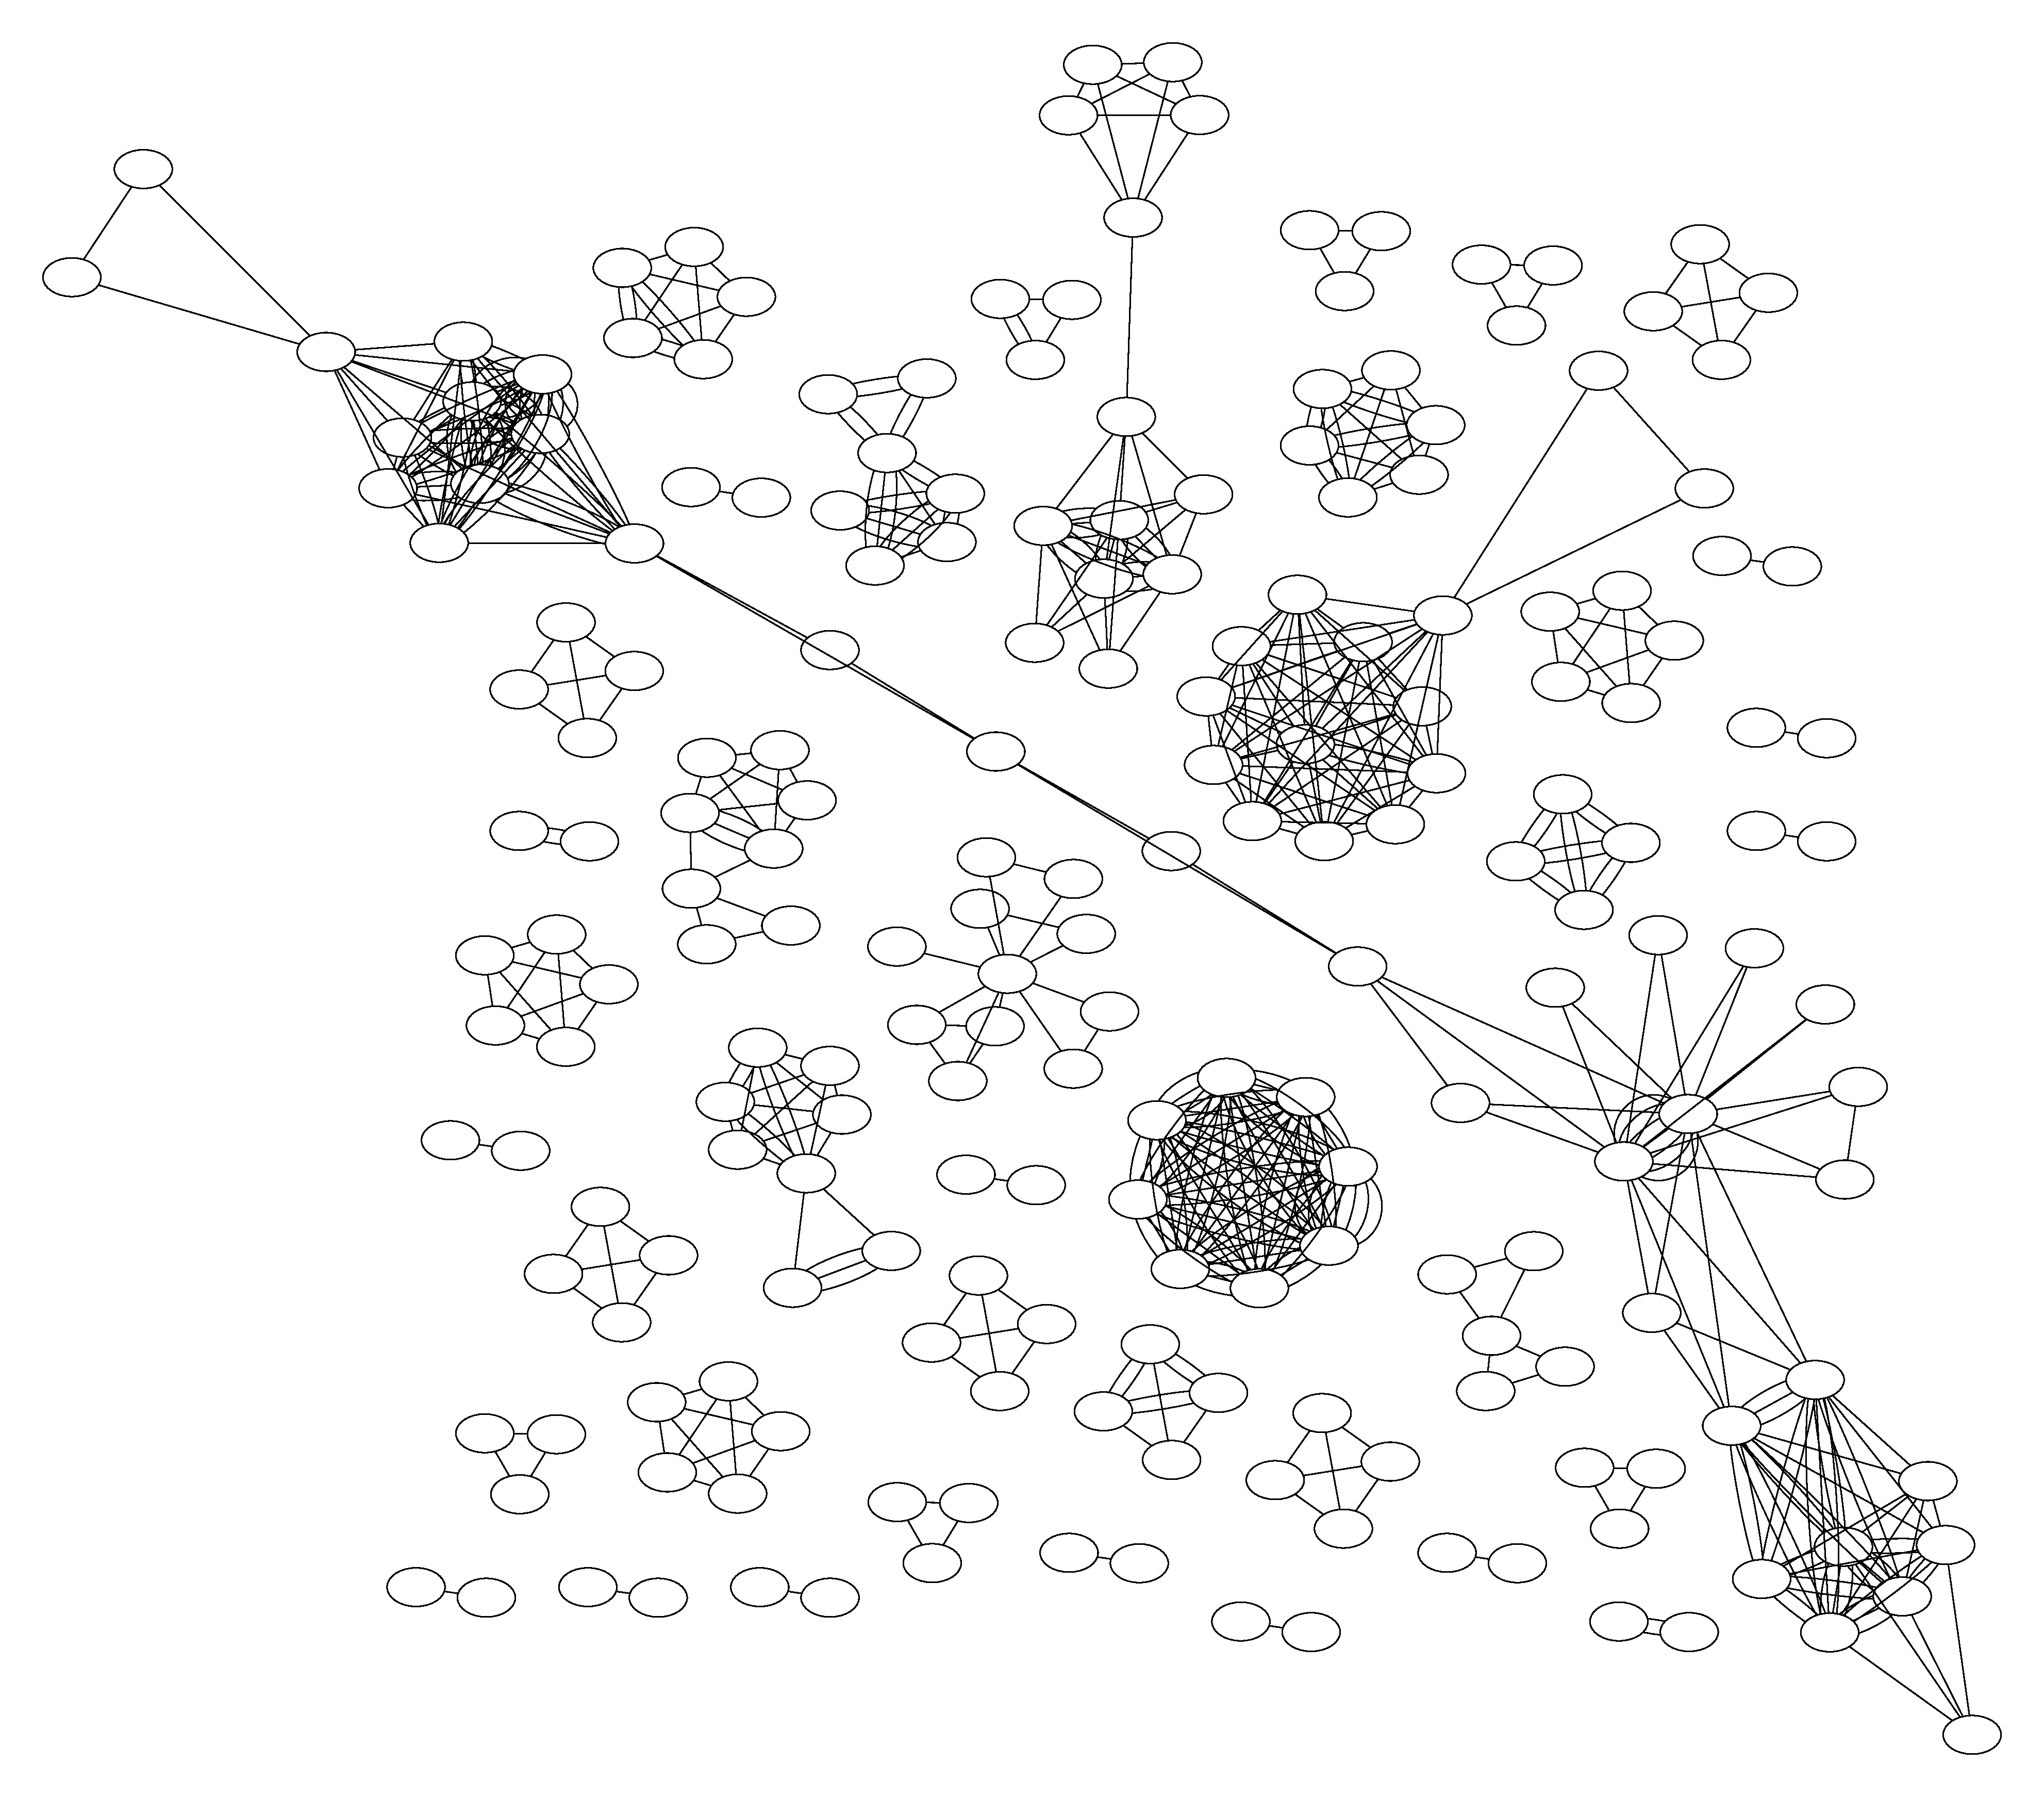
\includegraphics[width=\textwidth]{penguiconconflict}
	\vspace{-.5in}
	\label{fig_pc2013_graph}
\end{figure}

\subsection{Model for the Extended Conference Timetable Decision Problem}

Before describing the model for the PCO problem, we give an integer programming model where feasible solutions determine values of functions $f$ which correspond directly to schedules that satisfy the constraints laid out in the ECTTD decision problem.
We note that the size of $f$, i.e. the number of variables in our model, can be very large when building models corresponding to our application data.
\begin{gather*}
	\text{size of } f = \text{\# of presenters } \times \text{ \# of talks } \times \text{ \# of hours } \times \text{ \# of rooms }
\end{gather*}
For PC2013, $\text{size of } f = 193 \times 253 \times 37 \times 15 = $ 27,421,440. 
This number of variables could be problematic computationally, however, we know that many (nearly all) of these variables will be zero based on information we have at formulation time. 
For example, if a presenter $i$ doesn't give talk $j$, then $f(i,j,h,r) = 0$ for all $h \in H, r \in R$. 
Although integer programming solver may automatically fix such variables to zero in the preprocessing phase, we exclude these variables from the model at the time of construction.
We create an index set  $\mathcal F \subseteq \{1,\cdots,n\} \times \{1,\cdots,m\} \times H \times R$ where $f_{i,j,h,r} \in \mathcal F $ only if presenter $i$ gives talk $j$, the talk $j$, presenter $i$ and room $r$ are available at hour $h$, and room $r$ is suitable for the $j$th talk. 
In addition to this condition, we restrict the inclusion of variable indices in $\mathcal F$ to the intersection of the available hours of all \emph{co-presenters} (pairs of presenters that give the same talk), e.g. if co-presenters $i,i'$ have availability sets $\{h_2,h_3\}$ and $\{h_3,h_4\}$ (assuming room and talk availability is at least $\{h_2, h_3, h_4\}$) then only variables with $h=h_3$ for these co-presenters and talk will be included. 
In practice, the reduction of our solution space to only $\mathcal F$ gives a massive performance gain. 
For PC2013, this immediately reduced the number of variables down to 91,514 (a reduction of 99.997\%).

The variables indexed by $\mathcal F$ can be thought of as a sparse representation of the interesting elements of the domain of $f$. 
In addition to $\mathcal F$ we will use the index set $\mathcal G$ to represent tuples $(j,h,r)$ for which talk $j$ can be given by any presenter at hour $h$ in room $r$, and variables $g_{j,h,r}$ will indicate whether or not this occurs.
We will now describe a formulation that implements each of the constraints on $f$ in ECTTD.
\begin{quote}
	\textbf{ECTTD formulation}
	\begin{flalign}
		&\text{minimize: } 0& \\
		&\text{subject to:}&\\
		&\sum_{h,r: (i,j,h,r)\in \mathcal F} f_{i,j,h,r} = G_{ij}& \text{for every presenter $i$ and talk $j$}\label{ectto_ip_constraint_b}\\
		&f_{i,j,h,r} - f_{i',j,h,r} = 0\label{ectto_ip_constraint_c_2}& \text{for every talk $j$ with co-presenters $i$, $i'$}\\
		&\sum_{j,r: (i,j,h,r)\in \mathcal F} f_{i,j,h,r} \le 1& \text{for every presenter $i$ and hour $h$ }\label{ectto_ip_constraint_d}\\
		&\left(\sum_{i: (i,j,h,r)\in \mathcal F} f_{i,j,h,r}\right) - U \times g_{j,h,r} \le 0& \text{for each $g_{j,h,r} \in \mathcal G$} \label{ectto_ip_constraint_e_1}\\
		&\sum_{j: (j,h,r)\in \mathcal G} g_{j,h,r} \le 1& \text{for each hour $h$ and room $r$}\label{ectto_ip_constraint_e_2}\\
		&\text{binary: } f_{i,j,h,r}, g_{j,h,r}
	\end{flalign}
\end{quote}
The first requirement (a) of ECTTD merely enforces all availability and suitability sets. 
We implicitly enforce this in our model by considering only the variables indexed over $\mathcal F$. 
As such, no specific constraints are needed in our model.

The second requirement (b) ensures that every presenter is scheduled for all of their talks, which we receive as parameter $G$ to ECTTD where $G_{ij}$ is the number of times presenter $i$ should give talk $j$. 
For each presenter $i$ and talk $j$, the sum of the times they are scheduled (over all hours and rooms) should be $G_{ij}$; this is constraint \eqref{ectto_ip_constraint_b}.

To ensure requirement (c) we force that all co-presenters have the same schedule for their shared talk (constraint \eqref{ectto_ip_constraint_c_2}).

Requirements (a)-(c) guarantee that all presenters are scheduled for their talks and that co-presenters are scheduled together. 
Requirement (d) ensures that if a presenter has multiple talks, then these talks are scheduled during different hours.  
For each presenter $i$ and hour $h$, the sum of their schedule variables for their talks in all rooms must be less than or equal to one (constraint \eqref{ectto_ip_constraint_d}).

The final requirement (e) ensures that room scheduling is exclusive. 
We would like to simply iterate over $\mathcal F$ for a particular pair of hour $h$ and room $r$, summing all of these together. 
If we didn't allow co-presenters (like TTD) then we could simply make this sum less than or equal to one. But, for talks with co-presenters this sum varies. 
To overcome this we create indicator variables $g_{j,h,r}$ where $g_{j,h,r}=1$ whenever talk $j$ is scheduled at hour $h$ in room $r$; 
this is modeled in constraint \eqref{ectto_ip_constraint_e_1}, where $U$ represents a sufficiently large number.
Finally, constraint \eqref{ectto_ip_constraint_e_1} ensures that no room is multi-booked by checking the sum of $g_{j,h,r}$ for each pair $h,r$.

Solving this feasibility problem proved tractable. 
We solved this formulation with the open source IP solver CBC on PC2013 with varying numbers of talks pruned out to see how the model scales. 
The results are given in Figure \ref{ectto_run_time}.
\begin{figure}[h!]
	\caption{Run time of ECTTD model}
	\centering
	\input ecttd_model_run_time
	\label{ectto_run_time}
\end{figure}

\subsection{Model for the Preference Conference Optimization Problem}
We now turn our attention to the Preference Conference Optimization (PCO) problem. 
PCO adds an additional layer of complexity to ECTTD by including a matrix of preferences for attendees with the goal of minimizing the number of conflicts caused by concurrent talks. 
Through experimentation we have found that considering these preferences significantly increases the difficulty of solving our conference scheduling problem. 
We now present an integer programming model for PCO.

The PCO model we present builds on our previous ECTTD model. 
In addition to the $G$ variables which collapse the four dimensional $f$ function down to three dimensions ($\text{talk} \times \text{hour} \times \text{room}$), all the while considering only those variables for which a feasible schedule is even possible given the different availability constraints, we will introduce three new classes of variables for PCO. 
The first is $z$ which will collapse $g$ to two dimensions ($\text{talk} \times \text{hour}$). 
Next, we will expand $z$ to $c$ which will have a three dimensional range from $\text{talk} \times \text{talk} \times \text{hour}$; it will indicate if two talks $j, j'$ are given concurrently at hour $h$. 
%The final variable is $c$, which has the same dimensions and will represent the conflicts (calculated from $W$, the preference matrix) if $j, j'$ are both scheduled at $h$. 
As with previous models, the corresponding script (e.g. $\mathcal Z$ for $z$) will represent the index set of variables that are possible given availability constraints. 
The parameter $w$ is constructed from $W$ as a $\text{talk} \times \text{talk} \times \text{hour}$ matrix where each entry is the number of attendees who wish to attend both talks $j,j'$ for all $h$ when $j,j'$ can be given based on talk, presenter, and room availability. 
Formally, $w_{j,j',h} = |\{e_k \in E \; : \; e_k \text{ has } W_{kj} = 1 \text{ and } W_{kj'} = 1 \}|$ for each $h$ where $(h,j)\cup(h,j') \subseteq \mathcal{Z}$. 
The objective function that is minimized in the model is the sum of elements in $c$.
\begin{quote}
	\textbf{PCO formulation}
	\begin{flalign}
		&\text{minimize: } \sum_{(j,j',h) \in \mathcal C} w_{j,j',h} \times c_{j,j',h}& \label{pco_ip_objective} \\
		&\text{subject to:}&\\
		&\sum_{h,r:(i,j,h,r) \in \mathcal F} f_{i,j,h,r} = G_{ij}& \text{for every presenter $i$ and talk $j$}\label{pco_ip_constraint_b}\\
		&f_{i,j,h,r} - f_{i',j,h,r} = 0\label{pco_ip_constraint_c_2}& \text{for every talk $j$ with co-presenters $i$, $i'$}\\
		&\sum_{j,r:(i,j,h,r) \in \mathcal F} f_{i,j,h,r} \le 1& \text{for every presenter $i$ and hour $h$ }\label{pco_ip_constraint_d}\\
		&\left(\sum_{i: (i,j,h,r)\in \mathcal F} f_{i,j,h,r}\right) - U \times g_{j,h,r} \le 0& \text{for each $(j,h,r) \in \mathcal G$} \label{pco_ip_constraint_e_1}\\
		&\sum_{j: (j,h,r) \in \mathcal G} g_{j,h,r} \le 1& \text{for each hour $h$ and room $r$}\label{pco_ip_constraint_e_2}\\
		&\left(\sum_{j,h: (j,h,r)\in \mathcal G} g_{j,h,r}\right) - U \times z_{j,h} \le 0& \text{for each room $r$}\label{pco_ip_constraint_z}\\
		&\sum_{h:(j,h) \in \mathcal Z} z_{j,h} = G_{ij}& \text{for each talk $j$ \text{ and some presenter $i$}}\label{pco_ip_constraint_z_2}\\
		&z_{j,h} + z_{j',h} -  c_{j,j',h} \le 1& \text{for each $  (j,j',h) \in \mathcal C$}\label{pco_ip_constraint_z'} \\
%		&c_{j,j',h} - w_{j,j',h} \times z'_{j,j',h} = 0& \text{for all $j,j',h \in \mathcal {Z'}$} \label{pco_ip_constraint_w}\\
		&\text{binary: } f_{i,j,h,r}, \; g_{j,h,r}, \; z_{j,h}, \; c_{j,j',h}&
%		&\text{integer: } c_{j,j',h}&
	\end{flalign}
\end{quote}
Constraints \eqref{pco_ip_constraint_b} - \eqref{pco_ip_constraint_e_2} are the same as in our model for ECTTD. 
Constraint \eqref{pco_ip_constraint_z} begins to build the $z$ variables which will be 0-1 indicators of talk $j$ being given at hour $h$ via the same boolean cast mechanism described previously by collapsing the room entries for $j,h$ in $g$. 
To ensure that only the correct number of $z$s are set to one, constraint \eqref{pco_ip_constraint_z_2} sums all hours $h$ for each talk $j$ and sets it equal to the number of times that talk $j$ was set to be given in the problem instance (the matrix $G$). 
It is of note that we pick \emph{any} presenter $i$'s entry in $G$ for talk $j$; although it is possible that a co-presenter $i'$ may have a different value for $G_{i'j}$ requirement (c) of PCO explicitly forbids this since it would be impossible for all co-presenters to be at all instances of a talk if they had different entries for their shared talk $j$, thus we can pick any presenter $i$.

The $z$ variables will now be used to generate $c$, which indicates if a pair of talks $j,j'$ are being given concurrently at hour $h$. 
Specifically, constraint \eqref{pco_ip_constraint_z'} , enforces that $z_{j,h} = 1 \text{ and } z_{j',h} = 1 \implies c_{j,j',h}=1$. 
The objective (\ref{pco_ip_objective}) of the model is to minimize the sum of RSVP conflicts.
Each variable $c_{j,j',h}$ appears with coefficient of $w_{j,j',h}$, which is the number of RSVP conflicts generated by talks $j$ and $j'$ being scheduled in the same time period.
Note that if the coefficient $w_{j,j',h}$ is nonzero, then the minimization nature of the problem will force the corresponding $c_{j,j',h}$ to take zero value whenever possible.

To measure the efficiency of our model we tested it on our sample set PC2013. 
This data set included information about talks, speakers and attendance, but did not include participant RSVP preferences (as they were not solicited that year), however we may use this data to generate reasonable instances by taking the historical attendance data as a basis for generating hypothetical RSVP preferences.
Attendance figures we recorded for each talk given at PC2013; a distribution of the attendance per talk is shown in Figure \ref{2013_attendance_distribution}.
\begin{figure}[h!]
	\caption{Distribution of attendance at PC2013}
	\centering
	\input 2013_attendance_distribution
	\label{2013_attendance_distribution}
\end{figure}
The sum of all attendance counts was 4101 \cite{pc2013_attendance} for around 1000 unique attendees. 
For the purposes of testing our model created a $W$ such that $\sum\limits_{i=0}^{n} W_{ij}$ was equal to the attendance count for that talk $j$, i.e. we created an ``RSVP" for each real talk attendance at PC2013. 
Since individual attendee attendance wasn't tracked (only totals were) we took some liberties in distributing the RSVPs across the attendees in our model. 
We first randomly spread the RSVPs over the attendees using a uniform distribution; that is, if talk $j$ had an attendance of 24 in PC2013 then 24 attendees were randomly chosen to attend this talk. 
We solved our model with commercial solver Gurobi which returned a solution with an objective value of 0 after 64 seconds, i.e. a schedule with absolutely no attendee conflicts.
All computations were run on a machine with 4 12-core Intel Xeon E5-2695 CPUs running at 2.4 GHz with 96 GB of RAM
%\footnote{PCO models were run on a machine with 4 12-core Intel Xeon E5-2695 CPUs running at 2.4 GHz with 96 GB of RAM. The authors would like to thank the SECS department at Oakland University for graciously providing the computation time for this paper. They would also like to thank Gurobi Optimization, Inc. for furnishing a free academic license of their Gurobi Optimizer.} .

After finding a non-conflicting schedule for uniformly distributed random attendees that followed the attendance counts in PC2013 we turned our attention to how the solver would react when the random attendees were not distributed uniformly. 
Our intuition was that, like the actual attendance figures, the distribution of attendance per attendee would not be evenly spaced out; there would be some attendees who went to many talks, and some who went to only a few. 
We chose a normal distribution with $\mu = 500, \sigma = 100$. 
For each attendance in the PC2013 distribution (Figure \ref{2013_attendance_distribution}) a random integer from the normal distribution was chosen. 
Since $\mu = 500$ those attendees with index around $500$ were much more likely to be chosen to RSVP to the talk then those with indices $50$ or $950$, which implemented our intuition that a small percentage of attendees will RSVP for many talks while the bulk of those remaining will RSVP to relatively few.
In addition, we added a check to ensure that no attendee was selected to attend more talks than were hours available; such a scenario would automatically preclude a zero objective value.
Even with an extremely powerful computer to run our model on and a state-of-the-art commercial solver we were unable to solve this instance after 24 hours. 
To help understand this phenomenon we created a half-sized problem (half as many talks and hours) and ran the model with decreasing values of $\sigma$ and found that the solving time exploded exponentially as $\sigma$ decreased; the average running time for $\sigma = 200$ was 22 seconds but increased to 22,683 seconds for $\sigma = 100$.

\subsubsection{Performance considerations}
After including RSVP preferences in our test models, the integer programming models became significantly more difficult to solve.
One possible cause of this is symmetry present in the models, a property that often leads to increased solution time \cite{sherali}.
An integer programming model is \emph{symmetric} if its variables can be permuted without changing the structure of the problem \cite{margot}. 
Our model exhibits high amounts of symmetry in relation to the scheduling of talks in rooms. 
If two rooms have the same availability and suitability set then permuting talk assignments among them in each hour produces no discernible change to the objective. 
It may be, however, that the solver will choose to branch early on in its branch-and-bound tree on these room assignments, leading to lots of unnecessary computation. 
In general it is difficult for the solver to detect that such variables ``really" represent the same thing, although there are several mechanisms for  determining and avoiding symmetry in solvers \cite{ostrowski}. 
However, it is easy for us to identify this symmetry and avoid it.

Two rooms will be said to be \emph{symmetric} if they have the same suitability and availability sets, i.e. for rooms $R_\alpha$ and $R_\beta$ we have that $R_\alpha$ and $R_\beta$ are symmetric if and only if
\begin{gather*}
	A_\alpha = A_\beta \quad \text{and} \\
	\{i \; | \; R_\alpha \in S_i \text{ for all } 1 \le i \le m\} = \{i \; | \; R_\beta \in S_i \text{ for all } 1 \le i \le m\}.
\end{gather*}
To break the symmetry we create room \emph{classes} which will represent several rooms with the same attributes. 
First, we make a new room set $R' = \{ r'=\{r_1, r_2, \cdots, r_p \}\subseteq R \; | \; \text{all } r \in r' \text{ are symmetric with each other} \}$. 
The corresponding new availability set $A'$ has simply the common availability set for each new $r' \in R'$. 
For the new suitability set $S'$ we replace each instance of $r$ with the room class $r'$ that $r$ is a member of. 
When we solve our model talks will be booked to room classes, avoiding the symmetry that arises by having to consider two essentially ``equal" rooms separately. 
When our model is solved we will have bookings in room classes, and we can arbitrarily assign the talk to any room in that class. 
We must make only one adjustment to our model: Constraint \eqref{pco_ip_constraint_e_2} in the PCO model ensures that each room has only one talk booked in it per hour. 
For our room classes we wish to relax this, requiring only that the number of bookings be at most the number of rooms in the class; this way, when we assign actual rooms from the solved model we can match talks to rooms in a one-to-one way. 
Formally, we will change constraint \eqref{pco_ip_constraint_e_2} to
\begin{gather}
	\sum_{j \in \mathcal G_{h,r}} g_{j,h,r} \le |r|.
\end{gather}
It is easy to see that this model degenerates to our regular PCO model when no rooms are symmetric; in this case each room class would contain only one room. 
In practice the removal of the room symmetries increased performance by roughly a factor of 5x for our solver on PC2013, which contained only three room classes but had fourteen rooms (see Figure \ref{2013_normal_sigma_run_time}). 

The next step we took to improve performance was to \emph{dualize} one class of constraints.
In this technique, these requirements are moved from being hard constraints in the model, to appearing in the objective function with a sufficiently large penalty to ensure their satisfaction.
We chose to dualize constraint (d), namely that no presenter is scheduled for more than one talk per hour. 
Intuitively, this seemed like a promising adjustment because these constraints are similar in structure to the RSVP conflicts that are minimized in the objective function.
We first created 0-1 indicator variables $d_{i,h} = 1 \iff $ presenter $i$ is doubly (or more) booked at hour $h$ by changing \eqref{pco_ip_constraint_d} (which enforced (d)) to
\begin{gather}
	\left( \sum_{j,r \in \mathcal F_{i,h}} f_{i,j,h,r} \right) - U \times d_{i,h} \le 1. \label{pco_ip_dualized_d}
\end{gather}
Where $U$ is a sufficiently large number.
The left hand side of \eqref{pco_ip_dualized_d} is the number of times that presenter $i$ is scheduled at hour $h$, and $d_{i,h}$ may be 0 or 1 if this sum is less than 2, but must be 1 if the sum is 2 or greater. 
We then changed the objective \eqref{pco_ip_objective} to 
\begin{gather}
	\text{minimize: } \sum_{(j,j',h) \in \mathcal C} w_{j,j',h} \times c_{j,j',h} + \sum_{(i,h) \in \mathcal D} U \times d_{i,h}.
\end{gather}
Our new objective places a penalty of $U$ on presenters being multiply booked.
We should choose $U$ sufficiently large so $d$ is identically zero, otherwise the model can be resolved with a larger value of $U$. 
In our experiments the dualized constraints were always satisfied after solving the model.
In practice, dualizing PCO led to moderate performance increases of roughly 75\% faster.

\begin{figure}[h!]	
	\caption{Run time of PCO model with decreasing $\sigma$}
	\centering
	\input 2013_normal_sigma_run_time \\
	\begin{tabular}{| l | r | r | r |}
		\hline
		 ($\sigma$) & Standard & Symmetry & Dualized \\ \hline
		 400 & 5.4 & 0.8 & 0.4 \\
		 350 & 10.0 & 1.2 & 0.4 \\
		 300 & 6.8 & 3.0 & 0.8\\
		 250 &12.8 &6.0 &2.2 \\
		 200 & 22.8 & 10.2 &2.0\\
		 150 & 196.2 & 156.8 & 45.2 \\
		 100 & 22683.7 & 4179.2 &3282.6 \\
		\hline
	\end{tabular}	
	\label{2013_normal_sigma_run_time}
\end{figure}

For a summary of solution times comparing the original model with the improved models discussed in this subsection see Figure \ref{2013_normal_sigma_run_time}. 
The three models compared are: the Standard model, which corresponds to the PCO formulation given by (9)-(15); the Symmetry model, which incorporates the symmetry breaking reformulation described above; and finally the Dualized model, which incorporates both the symmetry breaking reformulation, and the dualization of constraint (d) as described above.
The graph plots the average running time for solving 10 randomly generated instances for values of $\sigma$ between 100 and 400 with increments of 10. 
The table shows the same information, only listing times for instances where $\sigma$ is a multiple of 50.
All times are listed in seconds.
We also note that it turned out that for the generated instances solved in these experiments, the optimal solutions had an objective value of zero.


\section{Conclusion}\label{sec.conclusion}
Conference scheduling represents an important class of timetabling problems.
This paper studies a conference scheduling problem where participant RSVP conflicts are minimized, subject to a collection of hard constraints.
We have demonstrated integer programming to be an effective solution technique, especially after incorporating symmetry breaking and other improvements.
	
\begin{thebibliography}{9}
	\bibitem{even76}
	Even, S., A. Itai, and A. Shamir. 1976. On the complexity of timetable and multicommodity flow problems. SIAM Journal on Computing 5, (4) (12): 691-13
	\bibitem{garey76}
	Garey, M., and D. Johnson. 1976. Computers and Intractability: A Guide to the Theory of NP-Completeness. New York: W. H. Freeman
	\bibitem{lovelace2010}
	Lovelace, A. 2010. On the complexity of scheduling university classes. M.S. in Computer Science Thesis. California Polytechnic State University: U.S.A.	
	\bibitem{garey76_2}
	Garey, M., D. Johnson, and L. Stockmeyer. 1976. Some simplified NP-Complete graph problems. Theoretical Computer Science 1: 237-267
%	\bibitem{cheng}
%	Cheng, E., Kleinberg, S., Kruk, S., Lindsey, W., and D. Steffy 2004. A strictly combinational approach to a university exam scheduling problem. Congressus Numerantium 167: 121-132
	\bibitem{pc}
	Penguicon Conference, \texttt{http://www.penguicon.org/}, Accessed: January, 2015.
	\bibitem{pc2013_attendance}
	Penguicon Programming Ops. \texttt{http://penguicon.info/doku.php/programmingops?s=attendance}.  Accessed: January, 2015. %Retried November 6, 2014
%	\bibitem{scip}
%	Achterberg, T. 2009. SCIP: solving constraint integer programs. Mathematical Programming Computation, Volume 1, Number 1: 1-41
%	\bibitem{zimpl}
%	Koch, T. 2004. Rapid Mathematical Programming. Ph.D. Thesis. Technische Universit{\"a}t Berlin. Germany
	\bibitem{sherali}
	Sherali, H.D., and J.C. Smith. 2001. Improving Discrete Model Representations via Symmetry Considerations. Managements Science 47: 1396-1407.
	\bibitem{margot}
	Margot, F. 2009. Symmetry in Integer Linear Programming. 2010. 50 Years of Integer Programming 1958-2008, Chapter 16: 647-681. Springer.
	\bibitem{ostrowski}
	Ostrowski, J. 2008. Symmetry in Integer Programming. Ph.D. Thesis. Lehigh University: U.S.A. 
\end{thebibliography}
	
\end{document}
